\documentclass{article}
\usepackage{graphicx, caption} % Required for inserting images
\usepackage{babel}
\usepackage{polski}
\usepackage[a4paper, right=3cm]{geometry}
\usepackage[T1]{fontenc}
\usepackage{amsmath,amsthm,amssymb}
\usepackage[utf8]{inputenc}
\usepackage{amsmath}
\usepackage{array}
\usepackage{multicol}
\usepackage{multirow}
\usepackage{float}

\title{Sprawozdanie wyznacznie współczynnika lepkości}
\author{Jan Rolka, Aleksander Pyrdek, Aleksander Mystkowski}
\date{November 2024}

\begin{document}
\maketitle
\newpage

\section{Wstęp teoretyczny}

\vspace{0.5cm}

Przy przepływie wszystkich cieczy rzeczywistych ujawniają się większe lub mniejsze siły tarcia. W przeciwieństwie do ruchu ciał stałych, w którym tarcie występuje tylko na powierzchni, w cieczach i w gazach ujawnia się ono w całej objętości. Jest więc zwane tarciem wewnętrznym lub lepkością.

\vspace{0.5cm}

Współczynnik lepkości \(\eta\) jest miarą oporu, jaki ciecz stawia przepływowi. Opisuje on zależność między siłą ścinającą \(\tau\) a szybkością ścinania \(\dot{\gamma}\), zgodnie ze wzorem:
\[
\eta = \frac{\tau}{\dot{\gamma}}
\]
gdzie:
\begin{itemize}
    \item \(\tau\) — naprężenie styczne w cieczy [Pa],
    \item \(\dot{\gamma}\) — szybkość ścinania [s\(^{-1}\)].
\end{itemize}

\vspace{0.5cm}

Badanie lepkości cieczy polega na obserwacji ruchu kuli spadającej w płynie, zgodnie z prawem Stokesa. Siła oporu działająca na kulę jest proporcjonalna do współczynnika lepkości, jej średnicy oraz prędkości. Zależność ta wyraża się wzorem:
\[
F = 6 \pi \eta r v,
\]
gdzie:
\begin{itemize}
    \item \(F\) — siła oporu [N],
    \item \(r\) — promień kuli [m],
    \item \(v\) — prędkość kuli [m/s].
\end{itemize}

\vspace{0.5cm}

Pomiar współczynnika lepkości pozwala na charakteryzację właściwości fizycznych cieczy, takich jak jej płynność czy zdolność do tłumienia ruchu.


\section{Aparatura}

\begin{enumerate}
    \item Przyrząd do badania spadania kulki w cieczy (rys. w1)
    \item Zestaw kulek
    \item Śruba mikrometryczna
    \item Suwmiarka
    \item Waga cyfrowa
\end{enumerate}

\begin{figure}[h]
\centering
\captionsetup{width=.7\linewidth}
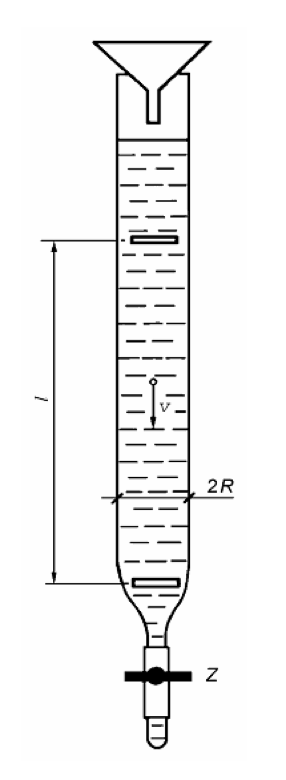
\includegraphics[scale=0.4]{rysunek1.png}
\caption{Rys. w1. Przyrząd do pomiaru współczynnika lepkości metodą Stokesa. (Z – zacisk służący do odzysku kulek)[1]}
\label{fig:example}
\end{figure}

\section{Wykonanie ćwiczenia}

\begin{enumerate}
    \item Wybrane do pomiaru kulki dokładnie wytarto z resztek gliceryny, a następnie rozłożono na arkuszu bibuły, jednocześnie nadano każdej z nich numer. Po wykonaniu jakiegokolwiek pomiaru, użyta kulka powinna zawsze zostać wytarta i odłożona na miejsce.
    
    \item Zmierzono średnice wszystkich wybranych kulek za pomocą śruby mikrometrycznej. Wyniki zapisano w Tabeli 1.
    
    \item Zważono wszystkie kulki przy użyciu dostępnej wagi. Wyniki zapisano w Tabeli 1.
    
    \item Ustawiono na rurze dwa znaczniki w odległości około 80 cm tak, aby górny znacznik znajdował się co najmniej 20 cm poniżej poziomu cieczy w rurze. Zanotowano odległość znaczników w Tabeli 1.
    
    \item Odczytano wartość średnicy używanego cylindra. Dane wpisano do Tabeli 1.
    
    \item Każdą z kulek wrzucono do rury, a następnie zmierzono za pomocą stopera czas, w którym będzie ona opadała pomiędzy znacznikami. Wynik zapisano w Tabeli 1. Zwrócono uwagę aby kulki opadały środkiem cylindra, a nie blisko ścianek oraz aby nie było do nich doczepionych pęcherzyków powietrza. Każdy pomiar, który nie spełnia powyższych wymogów powtórzono.
    
    \item Wyciągnięto kulkę z cylindra poprzez kran umieszczony na jego dolnym końcu. Aby nie dopuścić do wylewania się gliceryny z cylindra posłużono się zaciskaczem umieszczonym na wężyku. Gliceryna powinna ściekać do podstawionego pod wężykiem naczynia. Jeśli zachodzi potrzeba uzupełnienia gliceryny w cylindrze, należy przelać ją ostrożnie z naczynia lejąc po ściankach cylindra tak, aby wytworzyć jak najmniej pęcherzyków powietrza.
    
    \item Po skończonych pomiarach zanotowano temperaturę otoczenia, w której wykonywane było doświadczenie.[1]
\end{enumerate}



\section{Wyniki pomiarów:}
Droga spadania kulki = 800[mm]\\
Średnica cylindra = [mm]\\
Temperatura = 22.5[C]

\vspace{0.5cm}

\textbf{Tabela 1}
\begin{table}[h]
\begin{tabular}{|c|c|c|c|c|c|}
\hline
\begin{tabular}[c]{@{}c@{}}Nr\\ pomiaru\end{tabular} & \begin{tabular}[c]{@{}c@{}}Nr\\ kulki\end{tabular} & \begin{tabular}[c]{@{}c@{}}Średnica kulki\\ d [mm]\end{tabular} & \begin{tabular}[c]{@{}c@{}}Masa kulki\\ m [g]\end{tabular} & \begin{tabular}[c]{@{}c@{}}Czas spadku\\ kulki t [s]\end{tabular} & \begin{tabular}[c]{@{}c@{}}Wsp. lepkości\\ n [Pa * s]\end{tabular} \\ \hline
1                                                    & 1                                                  & 2.98                                                            & 0.110                                                      & 25.65                                                             &                                                                    \\ \hline
2                                                    & 2                                                  & 4.75                                                            & 0.443                                                      & 11.60                                                             &                                                                    \\ \hline
3                                                    & 3                                                  & 3.49                                                            & 0.176                                                      & 19.84                                                             &                                                                    \\ \hline
4                                                    & 4                                                  & 4.75                                                            & 0.443                                                      & 11.15                                                             &                                                                    \\ \hline
5                                                    & 5                                                  & 4.75                                                            & 0.444                                                      & 9.97                                                              &                                                                    \\ \hline
6                                                    & 6                                                  & 4.343                                                           & 0.176                                                      & 17.00                                                             &                                                                    \\ \hline
7                                                    & 7                                                  & 4                                                               & 0.266                                                      & 12.35                                                             &                                                                    \\ \hline
8                                                    & 8                                                  & 3.92                                                            & 0.266                                                      & 11.93                                                             &                                                                    \\ \hline
9                                                    & 9                                                  & 3                                                               & 0.109                                                      & 20.68                                                             &                                                                    \\ \hline
10                                                   & 10                                                 & 3                                                               & 0.113                                                      & 18.94                                                             &                                                                    \\ \hline
\end{tabular}
\end{table}

\section{Bibliografia}
[1] pf.agh.edu.pl

\end{document}
